    \documentclass{book}
\usepackage{graphicx}
    
    \begin{document}
       \parindent  0 pt
\parskip 5 pt
\input ../etc/def

       
{\bf  }

{\bf  }

{\tt  }

 

\title{{\sl \huge The Art of Computational Science}\\
\bigskip
{\sl Volume 1}\\
\bigskip
\bigskip
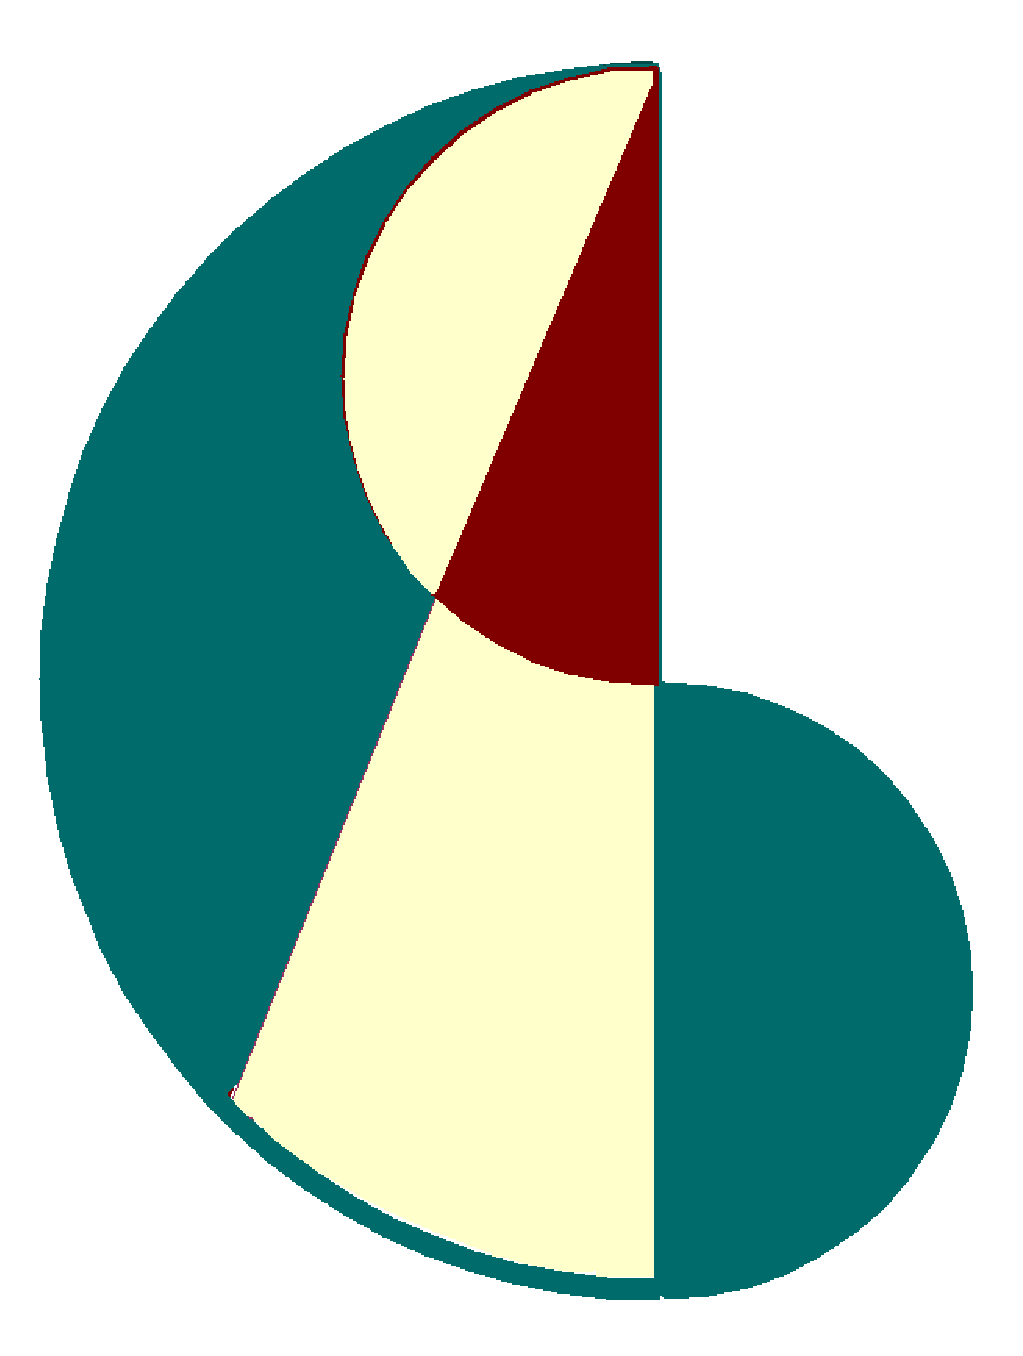
\includegraphics[width=3.5cm]{acstitle.ps}\\
\bigskip
\bigskip
\bigskip
\bf Moving Stars Around
\bigskip
}
\author{\bf Piet Hut, Jun Makino, Peter Teuben and Hans-Peter Bischof}


\maketitle
\thispagestyle{empty}
\chapter{  The Universe in a Computer}
\label{sect:3}

\section{  Gravity}
\label{sect:4}

Gravity is the weakest of all fundamental forces in physics, far
weaker than electromagnetism or the so-called weak and strong
interactions between subatomic particles.  However, the other three
forces lose out in the competition with gravity over long distances.
The weak and strong interactions both have an intrinsically short
range.  Electromagnetism, while being long-range like gravity, suffers
from a cancellation of attraction and repulsion in bulk matter, since
there tend to be as almost exactly as many positive as negative
charges in any sizable piece of matter.  In contrast, gravitational
interactions between particles are always attractive.  Therefore, the
more massive a piece of matter is, the more gravitational force it
exerts on its surroundings.

This dominance of gravity at long distances simplifies the job of
modeling a chunk of the Universe.  To a first approximation, it
is often a good idea to neglect the other forces, and to model the
objects as if they were interacting only through gravity.  In many
cases, we can also neglect the intrinsic dimensions of the objects,
treating each object as a point in space with a given mass.  All this
greatly simplifies the mathematical treatment of a system, by leaving
out most of the physics and chemistry that would be needed in a more
accurate treatment.

The objects we will be studying are stars, and the environment we will
focus on are dense stellar systems, star clusters where the stars are
so close together that they will occasionally collide and in general
have frequent interesting and complex interactions.  Some of the stars
can take on rather extremely dense forms, like white dwarfs and
neutron stars, and some stars may even collapse to form black holes.
However, in first approximation we can treat all these different types
of objects as point particles, as far as their gravitational
interactions are concerned.

We lay the groundwork for modeling a system of stars.  We start
absolutely from scratch, with a most simple code of less than a page
long.  In many small steps we then improve that code, pointing out the
many pitfalls along the way, on the level of programming as well as
astrophysical understanding.  We introduce helpful code development
facilities and visualization tools and give many hints as to how to
balance simplicity, efficiency, clarity, and modularity of the code.
Our intention is to introduce the topic from square one, and then to
work our way up to a robust set of codes with which one can do actual
research.  In later volumes in this series, we will continue to
develop these codes, adding many useful diagnostic tools, and
integrating those in a full production-level software environment.

\section{  Galactic Suburbia}
\label{sect:5}

Within the visible part of the universe, there are some hundred
billion galaxies.  Our galaxy is a rather typical spiral galaxy,
one of those many billions, and within our galaxy, our sun is a star
like any other among the hundred billion or so stars in our galaxy.

The sun is unremarkable in its properties.  Its mass is in
the mid range of what is normal for stars: there are others more than
ten times more massive, and there are also stars more ten times less
massive, but the vast majority of stars have a mass within a factor
ten of that of the sun.  Our home star is also unremarkable in its
location, at a distance of some thirty thousand light years from the
center of the galaxy.  Again, the number of stars closer to the center
and further away from the center are comparable.  Our closest neighbor,
Proxima Centauri, lies at a distance of a bit more than four light years.

This distance is typical for separations between stars in our neck of
the woods.  A light year is ten million times larger than the diameter
of the sun (a million km, or three light seconds).  In a scale model,
if we would represent each star as a cherry, an inch across, the
separation between the stars would be many hundreds of miles.  It is
clear from these numbers that collisions between stars in the solar
neighborhood must be very rare.  Although the stars follow random
orbits without any traffic control, they present such tiny targets
that we have to wait very long indeed in order to witness two of them
crashing into each other.  A quick estimate tells us that the sun has
a chance of hitting another star of less than  $10^{-16}$
per year.  In other words, we would have to wait at least
 $10^{16}$ years to have an appreciable chance to witness
such a collision.  Given that the sun's age is less than five Gigayears,
 $5.10^9$ years, it is no surprise that it does not show
any signs of a past collision: the chance that that would have
happened was less than one in a million.  Life in our galactic suburbs
is really quite safe for a star.

There are other places in our galaxy that are far more crowded, and
consequently are a lot more dangerous to venture into.  We will have
a brief look at four types of crowded neighborhoods: globular
clusters, galactic nuclei, star forming regions, and open clusters.

\section{  Globular Clusters}
\label{sect:6}


\renewcommand{\thefootnote}{\fnsymbol{footnote}}

 
\begin{figure}
\renewcommand{\thefootnote}{\fnsymbol{footnote}}
\renewcommand{\thempfootnote}{\fnsymbol{mpfootnote}}
\begin{minipage}{\columnwidth}
\begin{minipage}{\columnwidth}
\begin{center}
\renewcommand{\thefootnote}{\fnsymbol{footnote}}
    \includegraphics[width=10cm]{.imgs/1_m15.jpg.eps}
\caption{A snapshot of the globular cluster M15, taken with the
 {\it Hubble Space Telescope\protect \footnotemark[1]}.
}

\label{m15}
\end{center}
\renewcommand{\thefootnote}{\arabic{footnote}}
\end{minipage}
\renewcommand{\thefootnote}{\fnsymbol{footnote}}

\footnotetext[1]{\tt http://oposite.stsci.edu/pubinfo/PR/2000/25/content/0025y.jpg}

\end{minipage}
\end{figure}


 


In Fig. \ref{m15} we see a
picture of the globular cluster M15, taken with the Hubble Space
Telescope.  This cluster contains roughly a million stars.  In the
central region typical distances between neighboring stars are only a
few hundredths of a light year, more than a hundred times smaller than
those in the solar neighborhood.  This implies a stellar density that
is more than a million times larger than that near the sun.  Since the
typical relative velocities of stars in M15 are comparable to that of
the sun and its neighbors, a few tens of km/sec, collision times scale
with the density, leading to a central time between collisions of around
 $10^{10}$ years.  With globular clusters having an age of
roughly  $10^{10}$ years, a typical star near the center has
a significant chance to have undergone a collision in the past.  To be
a bit more precise, we don't know how long a typical star in the core
has remained in its current environment, but even if such a star has
been there only for a billion years, the chance of a collision has
already been  $\sim10\%$.

In fact, the chances are even higher than this rough estimate indicates.
One reason is the stars spend some part of their life time in a much
more extended state.  A star like the sun increases its diameter by
more than a factor of one hundred toward the end of its life, when
they become a red giant.  By presenting a much larger target to other
stars, they increase their chance for a collision during this stage
(even though this increase is partly offset by the fact that the red
giant stage lasts shorter than the so-called main-sequence life time
of a star, during which they have a normal appearance and diameter).
The other reason is that many stars are part of a double star system,
a type of dynamic spider web that can catch a third star, or another
double star, into a temporarily bound three- or four-body system.
Once engaged in such a tightly bound dance, the chance for collisions
between the stars is greatly increased.

A detailed analysis of all these factors predicts that a significant
fraction of stars in the core of a dense globular cluster such as M15
has already undergone at least one collision in its life time.  This
analysis, however, is quiet complex.  To study all of the important
channels through which collisions may occur, we have to analyze
encounters between a great variety of single and double stars, and
occasional bound triples and larger bound multiples of stars.  Since
each star in a bound subsystem can be a normal main-sequence star, a
red giant, a white dwarf, a neutron star or even a black hole, as well
as an exotic collision product itself, the combinatorial richness of
flavors of double stars and triples is enormous.  If we want to pick a
particular double star, we not only have to choose a star type for
each of its members, but in addition we have to specify the mass of
each star, and the parameters of its orbit, such as the semi-major axis
(a measure for the typical separation of the two stars) as well as the
orbital eccentricity.

\section{  Galactic Nuclei}
\label{sect:7}

In Fig. \ref{gc} we see an image of the very center of our galaxy.
This picture has been obtained with the Keck telescope,
in a near infrared wavelength band.


 
\begin{figure}
\begin{minipage}{\columnwidth}
\begin{center}
\renewcommand{\thefootnote}{\fnsymbol{footnote}}
    \includegraphics[width=10cm]{.imgs/2_gc.jpg.eps}
\caption{An image of the central region of our galaxy, as seen with the
 {\it Keck telescope\protect \footnotemark[1]}.
The massive black hole is located near the head of the arrow labeled
 ${\rm Sgr A}^*$.  The size of this image is two light
years by two light years, and the crowding is enormous: in the
neighborhood of the sun, typical distances between stars are several
light years, and a snapshot like this most likely would show just one
star or none at all.
}
 \footnotetext[1]{\tt http://www.astro.ucla.edu/$\sim$jlu/gc/pictures/lgs.shtml}

\label{gc}
\end{center}
\end{minipage}
\end{figure}



In the very center of our galaxy, a black hole resides with a mass a
few million times larger than the mass of our sun.  Although the black
hole itself is invisible, we can infer its presence by its strong
gravitational field, which in turn is reflected in the speed with
which stars pass near the black hole.  In normal visible light it is
impossible to get a glimpse of the galactic center, because of the
obscuring gas clouds that are positioned between us and the center.
Infrared light, however, can penetrate deeper in dusty regions.

In the central few light years near the black hole, the total mass of
stars is comparable to the mass of the hole.  This region is
called the galactic nucleus.  Here the stellar density is at least as
large as that in the center of the densest globular clusters.  However,
due to the strong attraction of the black hole, the stars zip around at
much higher velocities.  Whereas a typical star in the core of M15 has
a speed of a few tens of km/sec, stars near the black hole in the
center of our galaxy move with speeds exceeding a 1000 km/sec.
However, gravitational focusing is less by the same factor, and as a
consequence, the frequency of stellar collisions is comparable.

Modeling the detailed behavior of stars in this region remains a great
challenge, partly because of the complicated environmental features.
A globular cluster forms a theorist's dream of a laboratory, with its
absence of gas and dust and star forming regions.  All we find there
are stars that can be modeled well as point particles unless they come
close and collide, after which we can apply the point particle
approximation once again.  In contrast, there are giant molecular
clouds containing enormous amounts of gas and dust right close up to
the galactic center.  In these clouds, new stars are formed, some of
which will soon afterwards end their life in brilliant supernova
explosions, while spewing much of their debris back into the
interstellar medium.  Such complications are not present in globular
clusters, where supernovae no longer occur since the member stars are
too old and small to become a supernova.

Most other galaxies also harbor a massive black hole in their nuclei.
Some of those have a mass of hundreds of millions of solar masses, or
in extreme cases even more than a billion times the mass of the sun.
The holy grail of the study of dense stellar systems is to perform and
analyze accurate simulations of the complex ecology of stars and gas
in the environment of such enormous holes in space.  Much of the
research on globular clusters can be seen as providing the initial
steps toward a detailed modeling of galactic nuclei.

\section{  Star Forming Regions}
\label{sect:8}


 
\begin{figure}
\begin{minipage}{\columnwidth}
\begin{center}
\renewcommand{\thefootnote}{\fnsymbol{footnote}}
    \includegraphics[width=10cm]{.imgs/3_orion.jpg.eps}
\caption{The Orion Nebula, as seen by the
 {\it Subaru telescope\protect \footnotemark[1]}.
}
 \footnotetext[1]{\tt http://www.naoj.org/Science/press\_release/1999/01/Orion\_300.jpg}

\label{orion}
\end{center}
\end{minipage}
\end{figure}



There are many other places in the galactic disk where the density of
stars is high enough to make collisions likely, at least temporarily.
These are the sites where stars are born.  Fig. \ref{orion} taken by
the Japanese Subaru telescope in Hawaii shows the Orion Nebula, also
known as M42, at a distance of 1500 light years from the sun.  This
picture, too, is taking in infrared light in order to penetrate the
dusty regions surrounding the young stars.  These stars all recently
formed from the gas and dust that still surrounds them.

In order to study collisions in these star forming regions, we can no
longer treat the stars are point masses.  Many of the collisions take
place while the stars are still in the process of forming, before they
settle into their normal equilibrium state.  While a protostar is
still in the process of contracting from the gas cloud in which it was
born, it presents a larger target for collisions with other stars.  In
addition, a single contracting gas cloud may fission, giving rise to
more than one star at the same time.  In this way, the correlated
appearance of protostars is even more likely to lead to subsequent
collisions.

The proper way to model these processes is to combine gas dynamics and
stellar dynamics.  Much progress has been made recently in this area.
One way to use stellar dynamics in an approximate fashion is to begin
with the output of the gas dynamics codes, which present the positions
and velocities of a group of newly formed stars, and then to follow
and analyze the motions of those stars, including their collisions.

\section{  Open Clusters}
\label{sect:9}

Although stars are formed in groups, these groups typically do not
stay together for very long.  Perturbations from other stars and gas
clouds in their vicinity are often enough to break up the fragile
gravitational hold they initially have over each other.  Some of the
more massive groups of newly formed stars, however, are tightly bound,
enough to survive their environmental harassment.  They form the
so-called open clusters, where their name indicates that they have
central densities that are typically less than what we see in globular
clusters.


 
\begin{figure}
\begin{minipage}{\columnwidth}
\begin{center}
\renewcommand{\thefootnote}{\fnsymbol{footnote}}
    \includegraphics[width=10cm]{.imgs/4_m67.jpg.eps}
\caption{The open star cluster M67, in a picture taken at the 
 {\it Anglo-Australian Observatory\protect \footnotemark[1]}.
}
 \footnotetext[1]{\tt http://www.seds.org/messier/Pics/More/m67aat.jpg}

\label{m67}
\end{center}
\end{minipage}
\end{figure}



Fig. \ref{m67} shows one of the richest and densest open clusters, M67,
as observed by the Anglo-Australian Observatory.  Since this cluster
is old enough to have lost its gas and dust, all stars are visible at
normal optical wavelengths, at which this image is taken.  In the
central regions of this cluster, there are indications that some of
the stars have undergone close encounters or even collisions.  In
particular, some of the so-called blue stragglers may be merger
products.  Consequently, this star cluster qualifies as a dense
stellar system.

Open clusters typically have fewer members than globular clusters.
Also, they are younger.  Both facts makes it easier to simulate open
clusters than globular clusters.  On the other hand, the densest
globular clusters show a higher frequency and a far richer variety of
stellar collisions, making them a more interesting laboratory.  In
that sense, a dynamical simulation of an open cluster can be seen as
providing preparatory steps toward the modeling of globular clusters,
just as a study of the latter forms a stepping stone toward the
investigation of galactic nuclei.

\section{  Writing your own star cluster simulator}
\label{sect:10}

Astronomers have half a century of experience in writing computer
codes to simulate dense stellar systems.  The first published results
date back to 1960, and it was in the subsequent decade that it became
clear just how tricky it was to simulate a group of interacting stars.
The task seems so easy: for each star, just integrate Newton's
equations of motion (an object's acceleration is given by the applied
force divided by the mass of the object) under the influence of the
gravitational pairwise interactions of all other stars.  Indeed, it is
straightforward to write a simple code to do so, as we will see below.
And as long as all stars remain fairly well separated from each other,
even a simple code will do a reasonably good job.  For historical
reasons, this type of code is called an N-body code.

In practice, though, even a small group of stars will spontaneously
form one or more double stars.  This was discovered experimentally in
the early sixties.  One way to understand this result, after the fact,
is from an energetic point of view.  When a double star, or binary as
they are generally called, is formed, energy has to be released.  The
reason is that the two stars in a binary are bound, which means that
the total energy is negative, whereas two stars meeting each other
after coming in from far away have a positive net energy.  When
three stars come together randomly, there is a chance that two of the
three are left in a bound state, while the third one escapes, carrying
the excess energy.  Left by itself, a stellar system will exploit this
energy liberation mechanism by spontaneously forming binaries.

As soon as even one binary appears, a simple code with constant time
steps will give unacceptably large errors.  The first modification
needed is the introduction of an adaptive time step.  In the simplest
case, all particles will still share the same time step size, but that
size will change in time, in order to adequately resolve the closest
encounters between particles.  However, even a single binary can then
impose a tiny time step on the whole system, slowing everybody down.

By the end of the sixties, this problem was overcome by the
development of codes that employed individual time steps.  Stars with
close neighbors were stepped forward in time more frequently than
stars at large, and in this way the computational power was brought to
where it was most needed.

This modification in itself brought gravitational N-body codes already
well outside the range of systems that are normally discussed in text
books on numerical integration methods.  The internal book keeping
needed to write a correct and efficient code with individual time
steps is surprisingly large, given the simplicity of the task:
integrate the effect of pairwise attractive inverse square forces.
But this was only a first step toward the development of modern N-body
codes.  The presence of tight binaries produced much more of an obstacle,
and throughout the seventies a variety of clever mechanisms were developed
in order to deal with them efficiently.

For one thing, there are problems with round-off.  Two stars in a
tight orbit around each other have almost the same position vector, as
seen from the center of a star cluster, where we normally anchor the
global coordinate system.  And yet it is the separation between the
stars that determines their mutual forces.  When we compute the
separation by subtracting two almost identical spatial vectors, we are
asking for (numerical) trouble.  The solution is to introduce a local
coordinate system whenever two or more stars undergo a close
interaction.  This does away with the round-off problem, but it
introduces a host of administrative complexities, in order to make
sure that any arbitrary configuration of stars is locally presented
correctly -- and that the right thing happens when two or more of such
local coordinate patches encounter each other.  This may not happen
often, but one occurrence in a long run is enough to cause an
unacceptably large error if no precautions have been taken to deal
properly with such a situation.

We can continue the list of tricks that have been invented to allow
every larger and denser systems to be modeled correctly.  We will
encounter them later on, and explain them then in detail, but just to
list a few, here are some of the techniques.  Numerical problems with
the singularity in the two-body system have been overcome by mapping
two or more interacting stars from the three-dimensional Kepler
problem to a four-dimensional harmonic oscillator.  The total force on
particles has been split into different contributions, the first from
a near zone of relatively close neighbors and the second from a far
zone of all other particles, with each partial force being governed
with different integration time steps.  Tree codes have been used to
group the contributions of a number of more and more distant zones
together in ever larger chunks, for efficiency.  Triple stars have
received their own special treatment, especially the marginally stable
triples that are sometimes long-lived, but continuously changed their
inner state due to internal perturbations.  The list goes on.  See
Sverre Aarseth's book
 {\it Gravitational
N-Body Simulations\footnote{\tt http://www.cambridge.org/catalogue/catalogue.asp?isbn=0521432723}}

In this book, we will introduce a modern integrator, the Hermite
scheme, developed in the 1990s, together with a variable time step
integration scheme, where all stars share a common time step at any
given time.  Our emphasis will be on a complete explanation of all the
steps involved, together with a discussion of the motivation for those
steps.  In the last few chapters, we will embark on a research project
featuring stellar collisions, in a simple gravity-only approximation.

One of the roles of the current book is to provide an introduction to
the Kali code, and the other software tools that are part of the
 {\it Maya open lab\footnote{\tt http://www.ArtCompSci.org}}.  The Maya project
will make it possible to simulate an entire star cluster.

    \end{document}
